\documentclass[a4paper,11pt]{article}
% ============================================================================
%  PROJECT PROPOSAL — Focus Mode App
%  AWS First Cloud Journey (FCJ) Internship 2026
%  Author: Le Hoang Triet Thong (104171146)
%
%  NOTE: This file reuses the title-page / header-footer styling from the
%  author's LaTeX template. Compile with pdflatex (all packages below are
%  pdflatex-compatible). The body is written entirely in English.
% ============================================================================

% ---- Global layout & typography ----
\usepackage[utf8]{inputenc}
\usepackage[T1]{fontenc}
\usepackage{lmodern}
\usepackage{fancyhdr, graphicx, indentfirst, lastpage, setspace}
\usepackage{hyperref}
\usepackage{xurl} % allow long URLs to break across lines
\usepackage{float}
\usepackage{array, booktabs, multicol, multirow, siunitx, tabularx}
\usepackage{longtable}
\usepackage{enumitem}
\usepackage[table,dvipsnames]{xcolor}
\usepackage{tikz}
\usetikzlibrary{arrows.meta, positioning, shapes.geometric}
\usepackage{geometry}
\usepackage{tocloft} % Better control over Table of Contents
\usepackage{titlesec}

\geometry{
	top=0mm,
	bottom=0mm,
	left=0mm,
	right=0mm
}

\pagestyle{empty}

% ---- Colours (AWS-inspired, professional) ----
\definecolor{awsdark}{HTML}{232F3E}   % Squid ink
\definecolor{awsorange}{HTML}{EC7211}  % AWS orange
\definecolor{awsblue}{HTML}{1F6FEB}    % Interactive blue
\definecolor{tealaccent}{HTML}{0F766E}
\definecolor{rowgray}{HTML}{F2F4F6}
\definecolor{linkblue}{HTML}{15497B}

% ---- Section heading styling ----
\titleformat{\section}
  {\normalfont\Large\bfseries\color{awsdark}}{\thesection}{0.6em}{}
\titleformat{\subsection}
  {\normalfont\large\bfseries\color{awsorange!85!black}}{\thesubsection}{0.6em}{}
\titleformat{\subsubsection}
  {\normalfont\normalsize\bfseries\color{tealaccent}}{\thesubsubsection}{0.6em}{}

% ---- Hyperref ----
\hypersetup{
	colorlinks=true,
	linkcolor=linkblue,
	urlcolor=awsblue,
	citecolor=linkblue,
	pdftitle={Project Proposal - Focus Mode App},
	pdfauthor={Le Hoang Triet Thong}
}

% ---- Handy commands ----
\newcommand{\oosplit}{
	\begin{center}
		\begin{tikzpicture}
			\draw[line width=0.5 pt] (-4,0) -- (-0.3,0);
			\node at (0,0) {{\Large $\bullet$}};
			\draw[line width=0.5pt] (0.3,0) -- (4,0);
		\end{tikzpicture}
	\end{center}
}

% A boxed key-highlight callout
\newcommand{\keybox}[1]{%
	\begin{center}
	\fcolorbox{awsorange}{orange!6}{\parbox{0.94\linewidth}{\small #1}}
	\end{center}}

\renewcommand{\arraystretch}{1.25}
\setlist{itemsep=2pt, topsep=3pt}

\begin{document}

	% ==================== TITLE PAGE ====================
	\begin{tikzpicture}[remember picture,overlay]

		% Full-page background image
		\node[anchor=south west, inner sep=0] at (current page.south west) {
			
\includegraphics[width=\paperwidth,height=\paperheight]{Background/Background (1).png}
		};

		% --- Double frame ---
		\draw[line width=0.16 cm]
		([xshift=13mm,yshift=-13mm]current page.north west)
		rectangle
		([xshift=-13mm,yshift=13mm]current page.south east);

		\draw[line width=0.05 cm]
		([xshift=15mm,yshift=-15mm]current page.north west)
		rectangle
		([xshift=-15mm,yshift=15mm]current page.south east);

	\end{tikzpicture}

	\vspace*{15 mm}

	\begin{center}
		\textbf{\Large
			SWINBURNE UNIVERSITY OF TECHNOLOGY\\
		}

		\vspace*{4 mm}
		\textbf{\Large SCHOOL OF SCIENCE, COMPUTING}\\
		\vspace*{3 mm}
		\textbf{\Large AND ENGINEERING TECHNOLOGIES}
	\end{center}

	\oosplit

	\vspace{2 mm}
	\begin{center}
		
\includegraphics[scale=0.7]{Background/SUT.png}
	\end{center}
	\vspace*{2 mm}

	\begin{center}
		\begin{tabular}{c}
			\textbf{\Huge PROJECT PROPOSAL}         \\
			\\
			\textbf{\large Focus Mode App --- A Serverless, AI-Augmented}\\[2pt]
			\textbf{\large Productivity \& Well-being Platform on AWS}          \\
			\\
			\midrule
			\\
			\textbf{\large AWS First Cloud Journey (FCJ) Internship 2026}\\
			\bottomrule
		\end{tabular}
	\end{center}

	\vspace{0.7 cm}

	\begin{table}[h]
		\centering
		{\large
			\begin{tabular}{|p{8.2cm}|>{\centering\arraybackslash}p{3cm}|}
				\hline
				\multicolumn{1}{|c|}{\textbf{Full Name}} & \multicolumn{1}{c|}{\textbf{Student ID}} \\ \hline
				Le Hoang Triet Thong & 104171146 \\ \hline
			\end{tabular}
		}
	\end{table}

	\vspace{1.2 cm}

	\begin{center}
		\textbf{\large Ho Chi Minh City, 2026}
	\end{center}

	% ==================== RESET FOR CONTENT PAGES ====================
	\clearpage
	\newgeometry{top=2.5cm, bottom=2.5cm, left=2.5cm, right=2.5cm, headheight=15pt}

	\pagestyle{fancy}
	\fancyhf{}
	\lhead{\small Project Proposal --- Focus Mode App}
	\rhead{\small Le Hoang Triet Thong -- 104171146}
	\renewcommand{\headrulewidth}{0.4pt}
	\lfoot{\small AWS FCJ Internship 2026}
	\rfoot{\small Page \thepage\ of \pageref{LastPage}}
	\renewcommand{\footrulewidth}{0pt}

	\onehalfspacing
	\pagenumbering{arabic}

	% ==================== TABLE OF CONTENTS ====================
	\renewcommand{\contentsname}{\Large Table of Contents}
	\tableofcontents
	\clearpage

	% ============================================================
	% EXECUTIVE SUMMARY
	% ============================================================
	\section*{Executive Summary}
	\addcontentsline{toc}{section}{Executive Summary}
	\markboth{Executive Summary}{}

	Knowledge workers and students increasingly struggle to sustain deep focus in an
	environment engineered for distraction. Conventional Pomodoro timers address only the
	mechanics of time-boxing; they do nothing about the two factors that actually erode a
	work session: a distracting environment and the invisible emotional cost of the work
	itself. \textbf{Focus Mode App} is a cloud-native productivity and well-being platform
	that closes this gap. It combines an immersive focus timer with ambient sound, an
	AI task assistant, automatic post-session emotion detection, and emotion-aware content
	recommendations --- all delivered through a fully serverless architecture on Amazon Web
	Services (AWS) and Supabase.

	This proposal presents the solution's business rationale, its technical architecture,
	the implementation approach, a realistic delivery timeline, a detailed budget grounded
	in actual AWS pricing, a risk assessment, and the expected outcomes. Unlike a purely
	hypothetical proposal, every architectural decision and cost figure here is drawn from a
	working reference implementation: the system described has been built and deployed to a
	live production environment, so the numbers are measured rather than guessed.

	\medskip
	\noindent\textbf{Solution overview.} A single-page web application (Nuxt~3 / Vue~3),
	hosted on AWS Amplify, talks to a Supabase Backend-as-a-Service (PostgreSQL, Auth, and
	the \texttt{pgvector} extension) for all core CRUD and authentication. Five AI and media
	capabilities run as independent AWS Lambda functions behind an Amazon API Gateway HTTP
	API, using Amazon Bedrock for large-language-model reasoning (a Claude Haiku~4.5 task
	agent) and multilingual text embeddings (Cohere Embed Multilingual~v3). A sixth Lambda
	manages ambient-audio uploads to Amazon S3. Emotion detection runs a quantized DistilBERT
	model packaged directly inside its Lambda.

	\medskip
	\noindent\textbf{Key features:}
	\begin{itemize}
		\item Wall-clock-accurate Pomodoro focus timer with ambient audio streamed from S3.
		\item A conversational AI task assistant (Amazon Bedrock Agent) that creates, lists,
		      updates and deletes tasks from natural-language requests.
		\item Automatic emotion detection from a post-session journal entry (five labels).
		\item Retrieval-augmented (RAG) content recommendations matched to the detected emotion.
		\item Task management, a focus-history heatmap, downloadable worklog reports, an
		      in-app user guide, and a feedback channel.
		\item An admin CMS for user approval, media/embedding management, ambient-sound
		      management, and feedback triage.
	\end{itemize}

	\medskip
	\noindent\textbf{Business benefits and ROI.} The architecture is deliberately
	free-tier-first. At a representative pilot scale of ten users the measured operating cost
	is approximately \textbf{\$0.97 per month} (about \textbf{\$12 per year}), rising to no
	more than \textbf{\$1.51 per month} in the conservative worst case. Because the only
	unavoidable fixed costs are Amazon Bedrock (usage-based) and a single Route~53 hosted
	zone (\$0.50/month), the platform reaches positive ROI almost immediately: even a modest
	improvement in a single knowledge worker's focused output dwarfs an annual infrastructure
	bill smaller than the price of one lunch.

	\medskip
	\noindent\textbf{Investment and timeline.} The reference implementation was delivered by a
	single intern developer across a phased schedule of roughly nine weeks (backend
	foundation \(\rightarrow\) frontend and auth \(\rightarrow\) core focus/task features
	\(\rightarrow\) cloud AI services \(\rightarrow\) administration, hardening and
	documentation). Infrastructure investment is effectively zero; the dominant cost is
	developer time.

	\medskip
	\noindent\textbf{Success metrics and expected outcomes.} Success is measured by a working
	end-to-end focus loop (sign-in \(\rightarrow\) plan tasks \(\rightarrow\) focus with
	ambient sound \(\rightarrow\) journal \(\rightarrow\) emotion \(\rightarrow\)
	recommendation \(\rightarrow\) report), by all six AI/media Lambdas being live and
	verified end-to-end, and by keeping monthly cost under \$2 at pilot scale. These targets
	have been met in the reference build, which was internally assessed at 8.5/10 against a
	High-Distinction rubric. The strategic outcome is a reusable, well-architected serverless
	pattern --- managed BaaS for data plus event-driven AWS compute for AI --- that can be
	extended to other emotion-aware or agentic applications.

	\clearpage

	% ============================================================
	% 1. PROBLEM STATEMENT
	% ============================================================
	\section{Problem Statement}

	\subsection{Current Situation}
	The modern study-and-work environment is saturated with interruptions. Instant messaging,
	notifications, social feeds and context-switching between tools fragment attention into
	short bursts. The cost of a single interruption is not just the seconds it lasts: research
	on attention consistently shows that returning to a demanding task after an interruption
	takes many minutes of re-focus, and that frequent context switching measurably reduces the
	quality and volume of deep work. For students and knowledge workers whose output depends on
	sustained concentration, this is a direct productivity tax paid every day.

	At the same time, the tools people reach for to fight distraction are shallow. The typical
	Pomodoro or ``focus timer'' app does one thing: it counts down. It does not shape the
	working environment, it does not understand what the user is working on, and --- crucially
	--- it is blind to the user's psychological state. Burnout, frustration and loss of
	motivation build up silently across many sessions, and a bare countdown timer offers no
	way to notice or respond to them.

	\subsection{Key Challenges (Pain Points)}
	\begin{itemize}
		\item \textbf{Environmental distraction.} A plain timer does nothing to create an
		      immersive, low-distraction environment. Users still see a bright, busy screen and
		      hear whatever is around them.
		\item \textbf{Cognitive overhead of planning.} Turning a vague intention
		      (``prepare my CV'', ``revise for the exam'') into a concrete, ordered task list
		      is itself effortful, and that friction happens exactly when the user is trying to
		      start working.
		\item \textbf{Invisible emotional cost.} Most tools ask users to self-rate their mood on
		      a slider --- a step users skip or answer carelessly. The emotional signal that
		      would let the tool intervene (encourage a break, surface calming content) is never
		      captured reliably.
		\item \textbf{No supportive feedback loop.} When a user finishes a hard, draining
		      session, nothing responds to that. There is no mechanism that offers the right
		      encouragement or content at the moment it would actually help.
		\item \textbf{Fragmented history and reporting.} Focus data, task completion and mood
		      live in separate places, if they are recorded at all, so users cannot easily see
		      patterns or review a day's work.
		\item \textbf{Cost and operational burden for the builder.} For an individual developer
		      or a small team, standing up the servers, databases and AI infrastructure to
		      support these features traditionally means real recurring cost and real operations
		      work --- a barrier that keeps such tools from being built at all.
	\end{itemize}

	\subsection{Stakeholders Affected}
	\begin{itemize}
		\item \textbf{End users (students and knowledge workers).} The primary beneficiaries.
		      They want to enter deep focus quickly, be supported emotionally, and review their
		      progress --- without manual bookkeeping.
		\item \textbf{Administrators / content curators.} They approve users, curate the
		      knowledge base of supportive content (quotes, sutras, lecture transcripts,
		      videos), manage ambient audio, and read user feedback. They need a simple,
		      role-gated web console rather than direct database access.
		\item \textbf{The developer / operator.} Needs the whole system to run within free
		      tiers, deploy without heavyweight operations, and scale to zero when idle so that
		      an idle user base costs almost nothing.
	\end{itemize}

	\subsection{Business Consequences of Inaction}
	Without a solution, the productivity tax of fragmented attention continues unchecked, and
	the well-being dimension of focused work stays completely unaddressed by the existing crop
	of timer apps. From a builder's perspective, the alternative architectures are worse:
	a traditional always-on server incurs fixed monthly cost regardless of usage, requires
	patching and monitoring, and does not scale gracefully. Doing nothing therefore means
	either accepting an inferior user experience or accepting an operating model that is too
	expensive and too operationally heavy to justify for a small user base.

	\subsection{Market Opportunity}
	Productivity and focus applications are a large and growing category, and the differentiator
	that this proposal targets --- \emph{emotion-aware, AI-assisted} focus rather than a bare
	timer --- is still uncommon. The opportunity is to combine three modern capabilities that
	are now cheap to access individually: \\
	(1) managed Backend-as-a-Service for data and auth\\
	(2) serverless compute that scales to Zero\\
	(3) on-demand large-language-model and embedding APIs. Assembled correctly, these let a single developer ship a differentiated,
	AI-rich product at near-zero fixed cost --- an opportunity that did not exist a few years
	ago and that this proposal demonstrates is now realistic.

	\keybox{\textbf{Problem in one sentence:} existing focus tools count time but ignore the
	environment, the planning burden, and the user's emotional state --- and building a tool
	that addresses all three has, until recently, been too costly and operationally heavy for
	an individual to attempt.}

	% ============================================================
	% 2. SOLUTION ARCHITECTURE
	% ============================================================
	\section{Solution Architecture}

	\subsection{Architecture Overview}
	Focus Mode App uses an \textbf{event-driven, serverless, cloud-native} architecture built
	on two complementary platforms. \textbf{Supabase} provides the managed data plane ---
	PostgreSQL, authentication, and the \texttt{pgvector} vector store --- so that no database
	server has to be operated. \textbf{AWS} provides the compute and AI plane: a static web
	host (Amplify), DNS (Route~53), an HTTP API (API Gateway), six single-responsibility
	Lambda functions, and Amazon Bedrock for language-model reasoning and embeddings. Each
	component has one job, scales independently, and stays within free-tier limits at pilot
	scale. Figure~\ref{fig:arch} shows the as-built architecture.

	\begin{figure}[H]
		\centering
		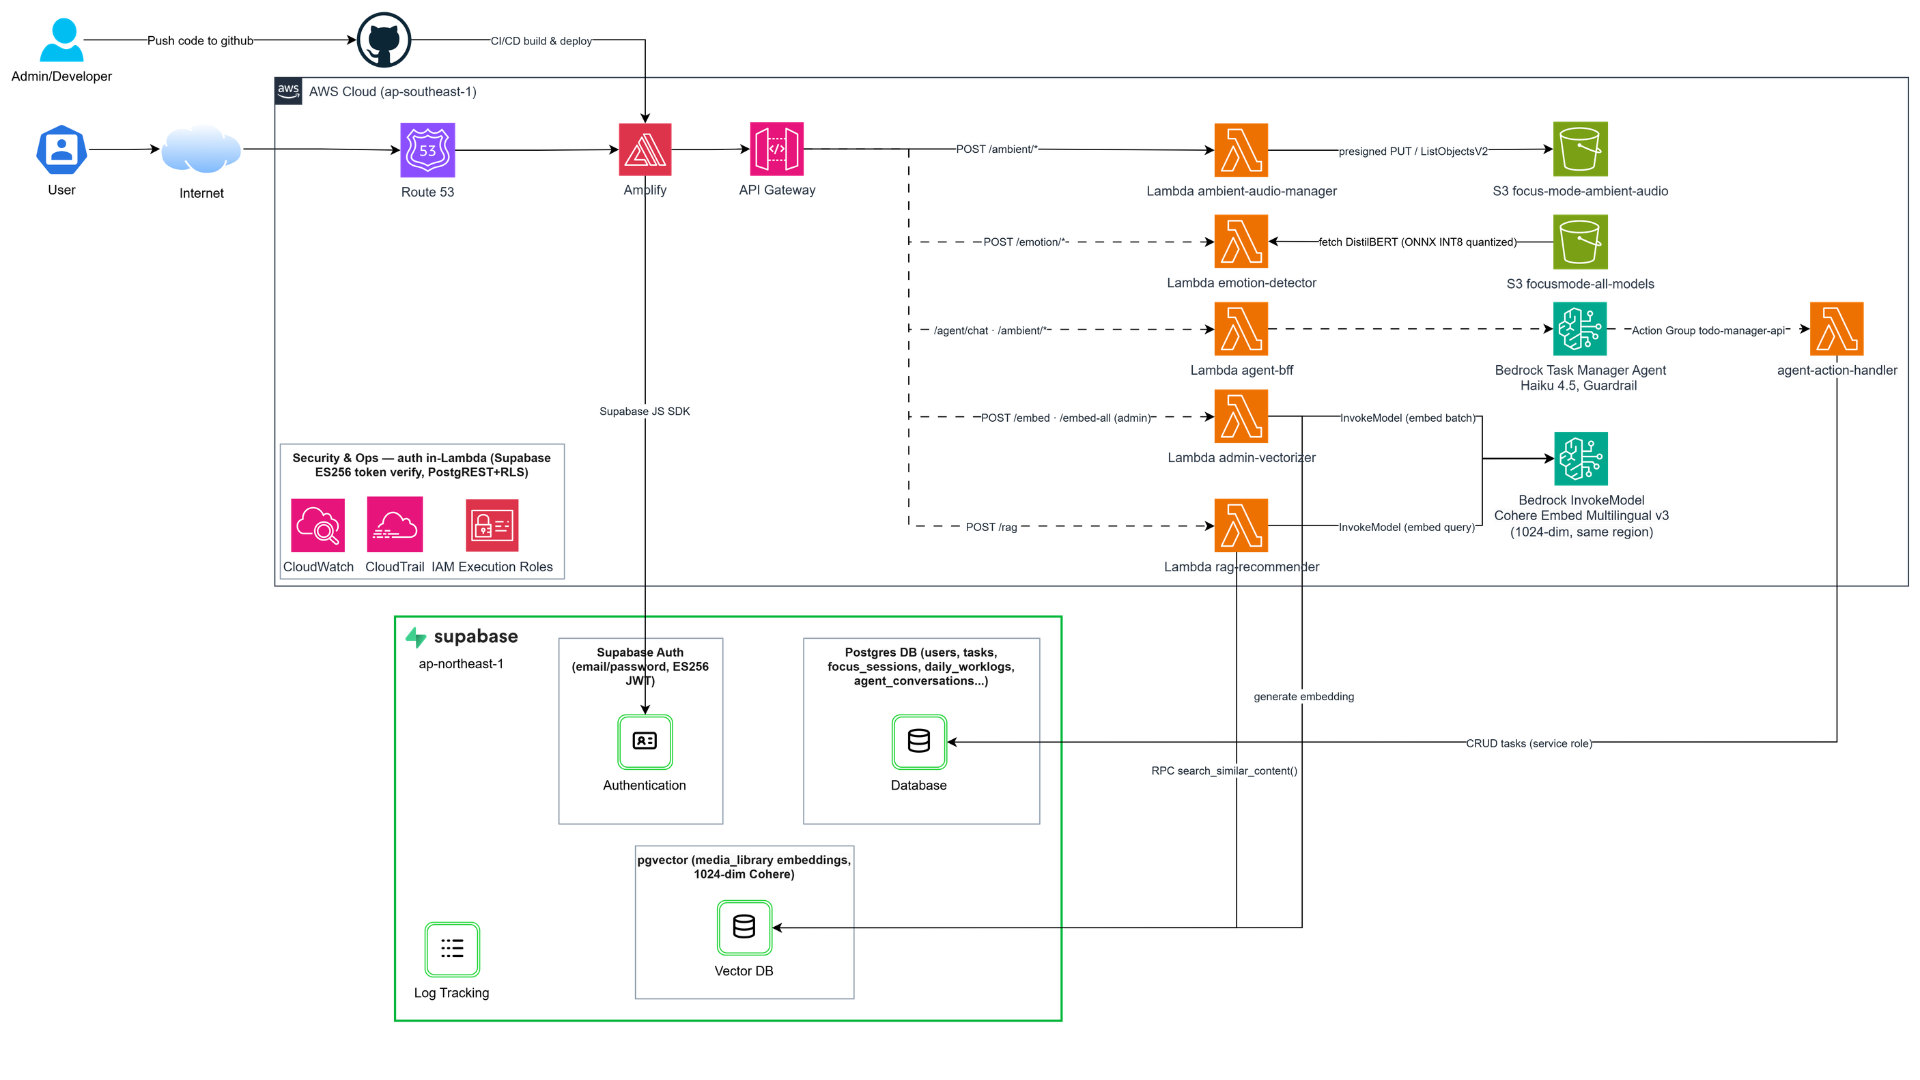
\includegraphics[width=\textwidth]{Background/Internship_Architecture.png}
		\caption{As-built architecture. The user's browser loads the Nuxt SPA from Amplify
		(via Route~53) and talks directly to Supabase for CRUD/auth; AI and media features are
		invoked through API Gateway to six Lambda functions, which call Amazon Bedrock and
		Supabase. Authentication is verified inside each Lambda against Supabase (ES256 +
		PostgREST + RLS).}
		\label{fig:arch}
	\end{figure}

	\subsection{AWS Services Used and Justification}
	Table~\ref{tab:services} lists each service and why it was selected over the alternatives.

	\begin{table}[H]
		\centering
		\footnotesize
		\rowcolors{2}{rowgray}{white}
		\begin{tabularx}{\textwidth}{@{}p{3.1cm} p{3.4cm} X@{}}
			\toprule
			\textbf{Service} & \textbf{Role in the system} & \textbf{Why this choice} \\
			\midrule
			AWS Amplify Hosting & Hosts the static Nuxt SPA; Git-based CI/CD & Zero-ops static hosting with a built-in build pipeline and generous free tier; no web server to manage. \\
			Amazon Route~53 & DNS for the custom domain & Native alias records to Amplify (free DNS queries); single hosted zone; integrates with the rest of AWS. \\
			Amazon API Gateway (HTTP API) & Single public entry point for all Lambda routes & HTTP API is cheaper and lower-latency than REST API; ample free tier; simple route-to-Lambda integration. \\
			AWS Lambda ($\times 6$) & Runs all AI/media logic, event-driven & Scales to zero (idle users cost nothing); per-request billing; 400{,}000 GB-seconds/month free \emph{perpetually}. \\
			Amazon Bedrock --- Agent (Claude Haiku~4.5) & Conversational task assistant & Managed LLM with tool-use/orchestration and guardrails; Haiku~4.5 gives the highest requests-per-minute quota available on the account (50~RPM) at low cost. \\
			Amazon Bedrock --- Cohere Embed Multilingual~v3 & Text embeddings for RAG \& vectorization & Available directly in \texttt{ap-southeast-1} (no cross-region call), 1024-dim, strong multilingual (incl. Vietnamese) quality; no inference profile needed. \\
			Amazon S3 & Ambient-audio files; ONNX model artifact & Cheap, durable object storage; presigned uploads keep credentials off the client. \\
			Amazon CloudWatch / CloudTrail & Logs, metrics, audit trail & Built-in observability for every Lambda; perpetual free log tier covers pilot scale. \\
			AWS IAM & Least-privilege execution roles & Scopes each Lambda to exactly the Bedrock/S3/logs actions it needs. \\
			\bottomrule
		\end{tabularx}
		\caption{AWS service selection and justification.}
		\label{tab:services}
	\end{table}

	\noindent\textbf{Why Supabase for the data plane.} Rather than run PostgreSQL on AWS (RDS),
	the design delegates the database, authentication and vector store to Supabase's managed
	free tier (500~MB database, 50{,}000 monthly active users, \texttt{pgvector} pre-enabled).
	This removes an entire class of operational work (backups, connection pooling, auth flows,
	Row-Level-Security enforcement) and keeps the AWS side focused purely on stateless compute
	and AI.

	\subsection{Component Design}
	The six Lambda functions each have a single responsibility:
	\begin{enumerate}
		\item \textbf{\texttt{agent-bff}} --- the ``backend for frontend'' for chat. It
		      authenticates the caller, injects the current date and a per-user session
		      namespace, and synchronously invokes the Bedrock Agent.
		\item \textbf{\texttt{agent-action-handler}} --- the Bedrock Agent's action group
		      (\texttt{todo-manager-api}). Bedrock calls it to \texttt{create}/\texttt{list}/
		      \texttt{update}/\texttt{delete} tasks; it writes to Supabase, always scoped to the
		      authenticated user.
		\item \textbf{\texttt{emotion-detector}} --- classifies journal text into one of five
		      labels (\emph{focused, stressed, exhausted, relaxed, unmotivated}) using a
		      DistilBERT model exported to ONNX and quantized to INT8, packaged directly inside
		      the Lambda.
		\item \textbf{\texttt{admin-vectorizer}} --- admin-only; generates Cohere embeddings for
		      media-library items (single or batch) and stores them in \texttt{pgvector}.
		\item \textbf{\texttt{rag-recommender}} --- maps a detected emotion to a query, embeds
		      it with Cohere, and runs a cosine-similarity search (\texttt{search\_similar\_content()})
		      to return the most relevant supportive content.
		\item \textbf{\texttt{ambient-audio-manager}} --- issues S3 presigned upload URLs and
		      lists ambient-audio objects for the admin console.
	\end{enumerate}

	\subsection{Data Model}
	All persistent state lives in Supabase PostgreSQL. Table~\ref{tab:datamodel} summarizes the
	main tables; the media-library table additionally carries a 1024-dimension
	\texttt{pgvector} column with an \texttt{ivfflat} cosine index.

	\begin{table}[H]
		\centering
		\footnotesize
		\rowcolors{2}{rowgray}{white}
		\begin{tabularx}{\textwidth}{@{}p{3.6cm} X@{}}
			\toprule
			\textbf{Table} & \textbf{Purpose} \\
			\midrule
			\texttt{users} & Mirrors \texttt{auth.users}; holds \texttt{role} and approval \texttt{status} (pending/approved/rejected). \\
			\texttt{tasks} & To-do items: status, priority, review, immutable \texttt{completed\_at}. \\
			\texttt{focus\_sessions} & Focus records: planned/actual duration, journal text, emotion label + confidence, ambient track. \\
			\texttt{daily\_worklogs} / \texttt{daily\_stats} & Aggregated daily focus statistics. \\
			\texttt{media\_library} & RAG content (quote/sutra/video/article/audio) with a \texttt{VECTOR(1024)} embedding. \\
			\texttt{ambient\_sounds} & Admin-managed ambient tracks (S3 URL, active flag, order). \\
			\texttt{agent\_conversations} / \texttt{agent\_messages} & Persisted AI chat history. \\
			\texttt{agent\_daily\_usage} & Per-user daily call counter for rate limiting. \\
			\texttt{feedback} & In-app user feedback (message, status new/read/resolved). \\
			\bottomrule
		\end{tabularx}
		\caption{Core data model (Supabase \texttt{public} schema).}
		\label{tab:datamodel}
	\end{table}

	\subsection{Security Architecture}
	Security is layered and does not rely on the client:
	\begin{itemize}
		\item \textbf{Authentication.} Supabase Auth issues \textbf{ES256}-signed JWTs. Because
		      API Gateway's built-in JWT authorizer supports only RS256, each Lambda verifies the
		      token \emph{in-function} by calling Supabase PostgREST with the caller's token; the
		      database then validates the signature and applies Row-Level Security. Admin routes
		      additionally check \texttt{role = 'admin'}.
		\item \textbf{Authorization at the data layer.} Row-Level Security (RLS) policies gate
		      every table so a user can only read/write their own rows; the \texttt{is\_admin()}
		      helper backs admin-only policies. A \texttt{BEFORE UPDATE} trigger blocks a user
		      from self-escalating their own \texttt{role}/\texttt{status}.
		\item \textbf{LLM safety.} The Bedrock Agent runs behind a \textbf{Guardrail}
		      (prompt-attack filtering at HIGH, denied topics) and a hardened system prompt that
		      treats user-supplied content as data, not instructions. The action handler enforces
		      a field whitelist and fail-closed user scoping to prevent confused-deputy and
		      mass-assignment attacks; the per-user session namespace prevents session hijacking.
		\item \textbf{Least privilege.} Each Lambda's IAM execution role grants only the specific
		      Bedrock/S3/logs actions it uses. Presigned S3 uploads keep bucket credentials off
		      the browser.
		\item \textbf{Abuse controls (at demo scale).} A per-user daily call limit
		      (\texttt{AGENT\_DAILY\_LIMIT}) and an input-size cap bound cost and abuse.
		      Network-edge rate limiting / WAF is intentionally out of scope at pilot scale (see
		      \S\ref{sec:risk}).
	\end{itemize}

	\subsection{Scalability and Performance}
	Because compute is serverless, throughput scales automatically with demand and falls to
	zero cost when idle --- the ideal profile for a bursty, per-user workload. Supabase's
	managed Postgres handles connection pooling and read scaling on the data side. The main
	performance considerations are Lambda cold starts (the emotion model adds a few seconds on
	a cold invocation but 1--2~seconds when warm) and the Bedrock Agent's requests-per-minute
	quota (Claude Haiku~4.5 provides 50~RPM, ample for pilot scale and raisable via Service
	Quotas). A known ceiling --- long multi-step agent operations approaching the API Gateway
	integration timeout --- is discussed as a risk in \S\ref{sec:risk}.

	\subsection{Representative Data Flows}
	\textbf{AI task assistant:} browser \(\rightarrow\) API Gateway \texttt{/agent/chat}
	\(\rightarrow\) \texttt{agent-bff} (auth + invoke) \(\rightarrow\) Bedrock Agent
	(Claude Haiku~4.5 + Guardrail) \(\rightarrow\) action group \texttt{agent-action-handler}
	\(\rightarrow\) Supabase \texttt{tasks} \(\rightarrow\) response streamed back to the chat UI.

	\smallskip
	\noindent\textbf{Emotion-aware recommendation:} on session end, the journal text is sent to
	\texttt{/emotion} \(\rightarrow\) \texttt{emotion-detector} returns a label + confidence
	\(\rightarrow\) the label is sent to \texttt{/rag} \(\rightarrow\) \texttt{rag-recommender}
	embeds a query (Cohere) and runs \texttt{search\_similar\_content()} over \texttt{pgvector}
	\(\rightarrow\) the top supportive items are shown to the user.

	% ============================================================
	% 3. TECHNICAL IMPLEMENTATION
	% ============================================================
	\section{Technical Implementation}

	\subsection{Implementation Phases and Deliverables}
	Implementation follows five incremental phases, each ending in a demonstrable deliverable:
	\begin{enumerate}
		\item \textbf{Backend foundation.} Provision Supabase; define the schema, triggers, and
		      RLS via sequential SQL migrations. \emph{Deliverable:} a secured database with a
		      working sign-up/approval flow.
		\item \textbf{Frontend and auth.} Scaffold the Nuxt~3 SPA; wire Supabase Auth,
		      route middleware (\texttt{auth}/\texttt{admin}) and the app shell.
		      \emph{Deliverable:} authenticated navigation across the core pages.
		\item \textbf{Core focus/task features.} Task CRUD with review, the wall-clock focus
		      timer, ambient audio, the post-session journal, and the history heatmap.
		      \emph{Deliverable:} the complete offline-of-mind focus loop, cloud-persisted.
		\item \textbf{Cloud AI services.} Implement and deploy the six Lambdas + Bedrock Agent;
		      wire the frontend composables with authenticated calls. \emph{Deliverable:} live
		      agent chat, emotion detection, and RAG recommendations.
		\item \textbf{Administration, hardening and documentation.} Admin CMS (users, media,
		      ambient, feedback), the user guide, security hardening, and the full document set.
		      \emph{Deliverable:} a production-ready, documented system.
	\end{enumerate}

	\subsection{Technical Requirements}
	\begin{itemize}
		\item \textbf{Compute:} six Python~3.12 Lambda functions; memory sized per function
		      (512~MB for the emotion model, less for the others). No always-on server.
		\item \textbf{Storage:} Supabase PostgreSQL (500~MB free tier is ample at pilot scale);
		      one S3 bucket for ambient audio and one artifact object for the ONNX model.
		\item \textbf{Network:} one API Gateway HTTP API with a route per Lambda; Route~53 alias
		      records to Amplify; all traffic over HTTPS.
		\item \textbf{External APIs:} Amazon Bedrock (Claude Haiku~4.5 agent; Cohere Embed
		      Multilingual~v3) in \texttt{ap-southeast-1}.
	\end{itemize}

	\subsection{Development Approach}
	The frontend is a Nuxt~3 single-page application (\texttt{ssr:false}) using Vue~3
	Composition API, Pinia stores (\texttt{task}, \texttt{focus}, \texttt{user}) for state, a
	set of composables (\texttt{useAuth}, \texttt{useDataService}, \texttt{useAgentChat},
	\texttt{useEmotionDetector}, \texttt{useRAG}, \texttt{useFeedback}, \dots) as the service
	layer, and Tailwind CSS for styling. Database evolution is managed through numbered,
	idempotent SQL migrations applied in order. Backend logic is plain Python with minimal
	dependencies, favouring direct calls to Bedrock and Supabase over heavy frameworks.

	\subsection{Key Implementation Decisions}
	Several decisions materially shaped the build and are worth calling out:
	\begin{itemize}
		\item \textbf{Cloud-only instead of offline-first.} The original concept called for an
		      offline-first client with a sync queue. This was deliberately dropped in favour of
		      a simpler cloud-only model (all reads/writes go straight to Supabase), removing an
		      entire class of conflict-resolution complexity for a single-user workload.
		\item \textbf{Claude Haiku~4.5 for the agent.} Selected because it offered the highest
		      requests-per-minute quota available on the account (50~RPM, versus single-digit RPM
		      for the alternatives), eliminating throttling on multi-turn conversations while
		      remaining fast and inexpensive.
		\item \textbf{Cohere Embed Multilingual~v3 for embeddings.} Chosen after verifying that
		      Amazon Titan embeddings are not available in \texttt{ap-southeast-1}; Cohere is
		      available in-region, is strongly multilingual, and needs no cross-region inference
		      profile.
		\item \textbf{DistilBERT ONNX in-Lambda for emotion.} Packaging a quantized model
		      directly in the function avoids a per-call Bedrock charge for a
		      high-frequency, low-complexity classification and keeps the feature self-contained.
		\item \textbf{In-Lambda ES256 auth.} Because Supabase tokens are ES256 and API Gateway's
		      JWT authorizer is RS256-only, verification was moved into each Lambda via PostgREST
		      + RLS --- a clean, defensible pattern rather than a workaround.
	\end{itemize}

	\subsection{Testing Strategy}
	The intended testing pyramid is: unit tests for critical logic (Pinia stores, the agent
	action handler's field-whitelisting, RLS-gated writes), integration tests against a test
	Supabase instance, and a small set of end-to-end tests covering the core loop
	(login \(\rightarrow\) task \(\rightarrow\) focus \(\rightarrow\) journal \(\rightarrow\)
	report). During development, each Lambda was verified end-to-end with real tokens via
	\texttt{curl} and CloudWatch inspection, and the frontend was type-checked
	(\texttt{nuxi typecheck}) as the gate before every commit. Automated regression coverage is
	an acknowledged gap that is deliberately scheduled last for the pilot (see \S\ref{sec:risk}).

	\subsection{Deployment Plan and Rollback}
	The frontend deploys automatically: a push to the GitHub repository triggers an Amplify
	build (\texttt{nuxt generate}) and release. Lambdas and the Bedrock Agent are deployed via
	documented AWS~CLI runbooks (package \(\rightarrow\) upload \(\rightarrow\) create/update
	function \(\rightarrow\) attach route). \textbf{Rollback} for the agent is built in: agent
	changes are versioned and served through an alias, so reverting is a matter of repointing
	the \texttt{prod} alias to a previous version; frontend rollback is an Amplify redeploy of a
	prior commit; database changes are forward-only migrations, so a corrective migration is the
	rollback path.

	\subsection{Configuration Management}
	Runtime configuration is entirely environment-driven: the frontend reads
	\texttt{NUXT\_PUBLIC\_*} variables (API base URLs, app URL) at build time; each Lambda reads
	its Supabase URL/keys and model IDs from environment variables. Secrets are held as Lambda
	environment variables at pilot scale (a managed secrets store is noted as a future
	hardening step, not required for a demo-scale deployment).

	% ============================================================
	% 4. TIMELINE & MILESTONES
	% ============================================================
	\section{Timeline \& Milestones}

	\subsection{Project Timeline}
	The project is delivered by a single intern developer over approximately nine working
	weeks, organised into the five phases from \S3. Table~\ref{tab:timeline} shows the schedule.

	\begin{table}[H]
		\centering
		\footnotesize
		\rowcolors{2}{rowgray}{white}
		\begin{tabularx}{\textwidth}{@{}p{1.6cm} p{3.2cm} X@{}}
			\toprule
			\textbf{Week} & \textbf{Phase} & \textbf{Focus of work} \\
			\midrule
			1 & Backend foundation & Supabase project, schema + migrations, auth trigger, RLS, user-approval flow. \\
			2 & Frontend \& auth & Nuxt SPA scaffold, Supabase Auth, route middleware, app shell. \\
			3--4 & Core features & Task CRUD + review, wall-clock focus timer, ambient audio, journal, history heatmap, dashboard. \\
			5--6 & Cloud AI services & Deploy six Lambdas + Bedrock Agent + Guardrail; wire authenticated frontend composables; verify each end-to-end. \\
			7--8 & Administration \& hardening & Admin CMS (users/media/ambient/feedback), user guide, security hardening, cost analysis. \\
			9 & Documentation \& submission & Full document set, architecture diagram, presentation, this proposal; final review. \\
			\bottomrule
		\end{tabularx}
		\caption{Nine-week delivery schedule.}
		\label{tab:timeline}
	\end{table}

	\subsection{Key Milestones}
	\begin{itemize}
		\item \textbf{M1 (end wk~1):} Secured database with working sign-up/approval.
		\item \textbf{M2 (end wk~2):} Authenticated SPA navigation.
		\item \textbf{M3 (end wk~4):} Complete focus loop, cloud-persisted --- the internal MVP.
		\item \textbf{M4 (end wk~6):} All AI features live and verified end-to-end.
		\item \textbf{M5 (end wk~8):} Admin CMS + hardening complete; production live.
		\item \textbf{M6 (end wk~9):} Documentation and submission package complete.
	\end{itemize}

	\subsection{Dependencies and Critical Path}
	The critical path runs schema \(\rightarrow\) auth \(\rightarrow\) core features \(\rightarrow\)
	AI services \(\rightarrow\) admin/hardening. The AI phase (M4) is the highest-risk link
	because it depends on external factors outside the codebase: Bedrock model access, RPM
	quotas, and correct IAM permissions. RAG additionally depends on the vectorizer (shared
	embedding dimension) and on the media library actually containing embedded content.

	\subsection{Resource Allocation and Buffer}
	Resourcing is a single developer, so phases run sequentially rather than in parallel;
	week~9 doubles as schedule buffer, absorbing spillover from the AI-integration phase (the
	most likely source of overrun). Because infrastructure is managed/serverless, there is no
	provisioning lead time to account for.

	% ============================================================
	% 5. BUDGET ESTIMATION
	% ============================================================
	\section{Budget Estimation}

	\subsection{Costing Assumptions}
	Costs are modelled for a representative pilot of \textbf{ten users} (2 active, 3 occasional,
	5 inactive), yielding roughly \textbf{52 focus sessions/month}. Within that, the assumed AI
	usage is: emotion detection once per session (52/month), agent chat on $\sim$40\% of
	sessions at $\sim$3 turns each ($\sim$63 turns/month), one RAG query per session (52/month),
	and $\sim$10 admin content embeddings/month. Token sizes are reasoned estimates (agent turn
	$\approx$ 1{,}500 input / 400 output tokens), not CloudWatch-measured figures, so a
	$\pm 2\times$ buffer is applied in the worst-case scenario. Prices were looked up from the
	official AWS pricing pages (July~2026), region \texttt{ap-southeast-1} where applicable.

	\subsection{Infrastructure Costs (Monthly)}
	Table~\ref{tab:budget} breaks down the monthly operating cost.

	\begin{table}[H]
		\centering
		\footnotesize
		\rowcolors{2}{rowgray}{white}
		\begin{tabularx}{\textwidth}{@{}X r p{5.2cm}@{}}
			\toprule
			\textbf{Service} & \textbf{\$/month} & \textbf{Notes} \\
			\midrule
			Bedrock --- Claude Haiku~4.5 (agent) & 0.22 & \$1/\$5 per 1M in/out tokens; usage-based; no free tier. \\
			Bedrock --- Cohere Embed Multilingual~v3 & $<$0.01 & \$0.10 per 1M input tokens; tiny at this scale. \\
			AWS Lambda ($\times 6$) & 0.00 & Well within the perpetual free tier (1M req + 400k GB-s). \\
			API Gateway (HTTP API) & 0.00 & Within free tier ($\sim$hundreds of req/month). \\
			Amazon S3 (ambient audio) & 0.00 & A few small MP3s; within free tier. \\
			CloudWatch Logs & 0.00 & Within the perpetual 5~GB free tier. \\
			AWS Amplify Hosting & 0.00 & $<$1~GB bandwidth + a few builds; within free tier. \\
			Supabase (Postgres/Auth/pgvector) & 0.00 & Free tier (500~MB DB, 50k MAU). \\
			Route~53 --- domain registration & 0.25 & Real purchase, $\sim$\$3/year amortized. \\
			Route~53 --- hosted zone & 0.50 & \$0.50/zone/month, fixed, no free tier. \\
			Route~53 --- DNS queries & $\sim$0.00 & Alias records to Amplify are free. \\
			\midrule
			\textbf{Total (standard)} & \textbf{$\approx$0.97} & $\approx$24{,}000~VND/month. \\
			\textbf{Total (worst case)} & \textbf{$\approx$1.51} & Free tiers expired + $2\times$ token buffer. \\
			\bottomrule
		\end{tabularx}
		\caption{Monthly infrastructure cost at a 10-user pilot scale.}
		\label{tab:budget}
	\end{table}

	\keybox{\textbf{Two facts drive this budget.} Only two cost groups have \emph{no} free tier:
	Amazon Bedrock (usage-based) and the Route~53 hosted zone (a fixed \$0.50/month regardless
	of traffic). Everything else fits inside free tiers at pilot scale --- and Lambda's free
	tier is \emph{perpetual}, while the API~Gateway and Amplify free tiers apply only for the
	first 12~months of the AWS account.}

	\subsection{Development and Operational Costs}
	The one-time development cost is developer time (approximately nine weeks of a single
	intern), not cash outlay. Ongoing operational cost beyond the table above is negligible:
	there are no servers to patch, no scaling to manage, and deployment is scripted. The only
	recurring cash cost is the sub-\$2/month infrastructure bill plus the annual domain renewal.

	\subsection{ROI and Break-Even Analysis}
	At pilot scale the annual infrastructure cost is roughly \textbf{\$12--18/year}. Framed
	against value, the break-even bar is trivially low: if the platform helps its users reclaim
	even a small amount of focused time per week, the value of that time vastly exceeds the
	cost. As an illustration (clearly a modelling assumption, not a measured result), if the
	tool saves each of ten users just 30~minutes of otherwise-lost time per week and that time
	is valued at even a modest hourly rate, the monthly value created is orders of magnitude
	larger than the $\sim$\$1 monthly cost --- so ROI is positive from the first month and
	break-even is effectively immediate. Should the product ever be commercialised, the same
	architecture supports a simple per-seat subscription whose marginal cost per user is a few
	cents of Bedrock usage, leaving a very high gross margin.

	\subsection{Cost-Optimization Strategies}
	\begin{itemize}
		\item \textbf{Free-tier-first design:} every component except Bedrock and the hosted zone
		      sits inside a free tier at pilot scale.
		\item \textbf{Scale-to-zero compute:} idle users incur no Lambda cost.
		\item \textbf{Model selection for cost:} Haiku (not a larger model) for the agent; a
		      self-hosted quantized model for the high-frequency emotion task instead of a
		      per-call API.
		\item \textbf{Input capping and batching:} capped input sizes bound token cost; the
		      vectorizer embeds up to a batch of items in a single Bedrock call.
		\item \textbf{In-region services:} choosing Cohere in \texttt{ap-southeast-1} avoids
		      cross-region data-transfer and latency.
	\end{itemize}

	% ============================================================
	% 6. RISK ASSESSMENT
	% ============================================================
	\section{Risk Assessment}
	\label{sec:risk}

	\subsection{Risk Matrix}
	Table~\ref{tab:risk} lists the principal risks with their likelihood, impact, and
	mitigation. Several of these are not hypothetical --- they were encountered and handled
	during the reference build.

	\begin{table}[H]
		\centering
		\footnotesize
		\rowcolors{2}{rowgray}{white}
		\begin{tabularx}{\textwidth}{@{}p{3.4cm} c c X@{}}
			\toprule
			\textbf{Risk} & \textbf{Likel.} & \textbf{Impact} & \textbf{Mitigation / contingency} \\
			\midrule
			Bedrock request throttling (RPM quota) & Med & Med & Use Haiku~4.5 (50~RPM, highest available); request a quota increase via Service Quotas if needed. \\
			Long agent operations time out (``Service Unavailable'') & Med & Med & Known API~Gateway $\sim$30s integration ceiling on large multi-step requests; contingency is to batch tool calls or move to an async invocation model. \\
			Free-tier expiry after 12 months (API GW, Amplify) & High & Low & Cost rises only marginally (cents); budgeted in the worst-case column. \\
			Embedding truncation ($>$2000 chars) & Med & Low & Cohere hard-limits input; long items embed on a prefix. Contingency: content chunking (\texttt{media\_chunks}). \\
			No automated test coverage yet & High & Med & Manual end-to-end verification + type-checking today; add unit/E2E tests on the riskiest paths first. \\
			Single-region / vendor dependence & Low & Med & Serverless design is portable; Supabase is standard Postgres; models are swappable behind the Lambda boundary. \\
			Secrets stored as plain env vars & Low & Med & Acceptable at demo scale; migrate to a managed secrets store before any real multi-tenant launch. \\
			Manual deploy (no IaC/CI for Lambdas) & Med & Low & Deployment runbooks are documented and repeatable; adopt SAM/CDK before scaling the team. \\
			\bottomrule
		\end{tabularx}
		\caption{Risk matrix (Likelihood / Impact / Mitigation).}
		\label{tab:risk}
	\end{table}

	\subsection{Mitigation and Contingency Summary}
	The design's biggest structural protection is that each risk is contained behind a clear
	boundary: models can be swapped behind a Lambda, the data layer is portable standard
	Postgres, and the frontend is a static bundle. The most material \emph{functional} risk ---
	the agent timing out on very large batch requests --- has a clear, understood remedy (batch
	the tool calls or invoke asynchronously) and does not affect normal single-action use.

	\subsection{Monitoring and Escalation}
	CloudWatch logs and metrics on every Lambda, plus CloudTrail for an audit trail, provide the
	visibility to detect throttling, errors and cost anomalies. At pilot scale, escalation is
	informal (the operator reviews logs and AWS Cost Explorer); a production launch would add
	alarms on error rate and spend.

	% ============================================================
	% 7. EXPECTED OUTCOMES
	% ============================================================
	\section{Expected Outcomes}

	\subsection{Success Metrics}
	\begin{itemize}
		\item \textbf{Functional:} the complete focus loop works end-to-end, and all six
		      AI/media Lambdas are live and verified (both achieved in the reference build).
		\item \textbf{Cost:} monthly operating cost stays under \$2 at pilot scale (achieved:
		      $\approx$\$0.97).
		\item \textbf{Quality:} the frontend type-checks cleanly and each Lambda is verified via
		      real-token end-to-end tests (achieved).
		\item \textbf{Assessment:} the reference build was internally assessed at \textbf{8.5/10}
		      against a High-Distinction rubric.
	\end{itemize}

	\subsection{Short-Term Benefits (0--6 months)}
	Users get an immersive, emotion-aware focus tool at essentially no infrastructure cost; the
	operator gets a live, documented, well-architected system that demonstrates managed BaaS +
	serverless AWS + Bedrock working together.

	\subsection{Medium-Term Benefits (6--18 months)}
	The architecture is a reusable template. Closing the acknowledged gaps --- automated tests,
	content chunking for long transcripts, and an async path for large agent operations ---
	would move the platform from a strong pilot to a genuinely production-grade product.

	\subsection{Long-Term Value (18+ months)}
	The pattern generalises well beyond this app: any product that needs managed data,
	scale-to-zero compute, and on-demand LLM/embedding capability can reuse it. Emotion-aware
	interaction and agentic task management are broadly applicable strategic capabilities. If
	commercialised, the near-zero marginal cost per user makes a high-margin subscription model
	viable.

	\subsection{User Experience Improvements}
	Compared with a conventional timer, the platform reduces the friction of planning (the AI
	assistant turns intentions into ordered tasks), makes the working environment immersive
	(ambient audio, focused UI), captures emotional signal automatically (no mood sliders), and
	closes the loop with supportive, relevant content --- a qualitatively different experience
	from ``a countdown on a screen''.

	% ============================================================
	% APPENDICES
	% ============================================================
	\clearpage
	\appendix
	\renewcommand{\thesection}{\Alph{section}}
	\section*{Appendices}
	\addcontentsline{toc}{section}{Appendices}

	\subsection{Appendix A --- Technical Specifications}
	\begin{itemize}
		\item \textbf{Frontend:} Nuxt~3 (\texttt{ssr:false}), Vue~3 Composition API, Pinia,
		      Tailwind CSS; deployed via \texttt{nuxt generate} to AWS Amplify.
		\item \textbf{Backend (data):} Supabase --- PostgreSQL, Auth (ES256 JWT),
		      \texttt{pgvector}; access governed by Row-Level Security and \texttt{is\_admin()}.
		\item \textbf{Backend (compute):} six Python~3.12 AWS Lambda functions behind one
		      API~Gateway HTTP API; per-function least-privilege IAM roles.
		\item \textbf{AI models (Amazon Bedrock, \texttt{ap-southeast-1}):} Claude Haiku~4.5
		      (agent, global cross-region inference profile, 50~RPM, behind a Guardrail);
		      Cohere Embed Multilingual~v3 (1024-dim embeddings). Emotion: DistilBERT exported to
		      ONNX, INT8-quantized, packaged in-Lambda; five labels (focused, stressed,
		      exhausted, relaxed, unmotivated).
		\item \textbf{API routes:} \texttt{/agent/chat}, \texttt{/emotion}, \texttt{/rag},
		      \texttt{/embed} \& \texttt{/embed-all} (admin), \texttt{/ambient/*}.
		\item \textbf{Regions:} AWS \texttt{ap-southeast-1} (Singapore); Supabase
		      \texttt{ap-northeast-1}.
	\end{itemize}

	\subsection{Appendix B --- Cost Calculation Detail}
	The per-service monthly figures in Table~\ref{tab:budget} derive from the usage model in
	\S5.1. Worked examples for the two paid groups:
	\begin{itemize}
		\item \textbf{Agent chat (Bedrock Haiku~4.5):} 63 turns $\times$ 1{,}500 input tokens
		      $= 94{,}500$ tokens $\approx 0.0945$M $\times$ \$1.00 $=$ \$0.0945 (input); 63
		      $\times$ 400 output $= 25{,}200$ tokens $\approx 0.0252$M $\times$ \$5.00 $=$
		      \$0.126 (output); total $\approx$ \textbf{\$0.22/month}.
		\item \textbf{Embeddings (Cohere Embed):} $\sim$52 RAG queries + $\sim$10 admin embeds,
		      a few thousand tokens total $\times$ \$0.10 per 1M $=$ well under one cent/month.
	\end{itemize}
	All other services fall within free tiers at this scale (see Table~\ref{tab:budget} notes).
	Figures are reasoned estimates, not production-measured; a one-month live run reconciled
	against AWS Cost Explorer would refine them.

	\subsection{Appendix C --- Architecture Diagram}
	See Figure~\ref{fig:arch} in \S2.1 for the full as-built architecture diagram (rendered at
	full width). It shows the end-to-end request flow from the user's browser through Route~53,
	Amplify, and API~Gateway to the six Lambdas, Amazon Bedrock, Amazon~S3, and the Supabase
	data plane, together with the security/operations layer (CloudWatch, CloudTrail, IAM,
	in-Lambda ES256 auth).

	\subsection{Appendix D --- References}
	\begin{enumerate}[label={[}\arabic*{]}]
		\item Amazon Web Services --- Bedrock pricing. \url{https://aws.amazon.com/bedrock/pricing/}
		\item Amazon Web Services --- Lambda pricing (perpetual free tier).
		      \url{https://aws.amazon.com/lambda/pricing/}
		\item Amazon Web Services --- API Gateway pricing.
		      \url{https://aws.amazon.com/api-gateway/pricing/}
		\item Amazon Web Services --- Amplify Hosting pricing.
		      \url{https://aws.amazon.com/amplify/pricing/}
		\item Amazon Web Services --- Route~53 pricing.
		      \url{https://aws.amazon.com/route53/pricing/}
		\item AWS Well-Architected Framework.
		      \url{https://aws.amazon.com/architecture/well-architected/}
		\item Supabase documentation --- Auth, PostgreSQL, and \texttt{pgvector}.
		      \url{https://supabase.com/docs}
		\item Cohere Embed Multilingual~v3 (via Amazon Bedrock) --- model documentation.
	\end{enumerate}

	\subsection{Appendix E --- Showcase Links}
	\begin{enumerate}[label={[}\arabic*{]}]
		\item Website link: \url{https://focusmode.click/}
		\item Presentation Slides: \url{https://canva.link/1a3sdbjvlyq0suq}
		
	\end{enumerate}

\end{document}
